\documentclass[14pt]{beamer}
\usepackage{./Estilos/BeamerUVM}
\usepackage{./Estilos/ColoresLatex}
%Sección para el tema de beamer, con el theme, usercolortheme y sección de footers
\usetheme{CambridgeUS}
\usecolortheme{default}
%\useoutertheme{default}
\setbeamercovered{invisible}
% or whatever (possibly just delete it)
\setbeamertemplate{section in toc}[sections numbered]
\setbeamertemplate{subsection in toc}[subsections numbered]
\setbeamertemplate{subsection in toc}{\leavevmode\leftskip=3.2em\rlap{\hskip-2em\inserttocsectionnumber.\inserttocsubsectionnumber}\inserttocsubsection\par}
\setbeamercolor{section in toc}{fg=blue}
\setbeamercolor{subsection in toc}{fg=blue}
\setbeamercolor{frametitle}{fg=blue}
\setbeamertemplate{caption}[numbered]

\setbeamertemplate{footline}
\beamertemplatenavigationsymbolsempty
\setbeamertemplate{headline}{}


\makeatletter
\setbeamercolor{secºtion in foot}{bg=gray!30, fg=black!90!orange}
\setbeamercolor{subsection in foot}{bg=blue!30!yellow, fg=red}
\setbeamercolor{date in foot}{bg=black, fg=white}
\setbeamertemplate{footline}
{
  \leavevmode%
  \hbox{%
  \begin{beamercolorbox}[wd=.333333\paperwidth,ht=2.25ex,dp=1ex,center]{section in foot}%
    \usebeamerfont{section in foot} \insertsection
  \end{beamercolorbox}%
  \begin{beamercolorbox}[wd=.333333\paperwidth,ht=2.25ex,dp=1ex,center]{subsection in foot}%
    \usebeamerfont{subsection in foot}  \insertsubsection
  \end{beamercolorbox}%
  \begin{beamercolorbox}[wd=.333333\paperwidth,ht=2.25ex,dp=1ex,right]{date in head/foot}%
    \usebeamerfont{date in head/foot} \insertshortdate{} \hspace*{2em}
    \insertframenumber{} / \inserttotalframenumber \hspace*{2ex} 
  \end{beamercolorbox}}%
  \vskip0pt%
}






% \usefonttheme{serif}
\usepackage[clock]{ifsym}
\usepackage{pstricks-add}
\DeclareSIUnit\erg{erg}
\DeclareSIUnit[number-unit-product = {\,}]\cal{cal}

\sisetup{per-mode=symbol}
\resetcounteronoverlays{saveenumi}

% Macro para agregar el logo de UVM en cada slide de la presentación

\addtobeamertemplate{frametitle}{}{%
\begin{tikzpicture}[remember picture,overlay]
\coordinate (logo) at ([xshift=-1.5cm,yshift=-0.8cm]current page.north east);
% \fill[devryblue] (logo) circle (.9cm);
% \clip (logo) circle (.75cm);
\node at (logo) {
\includegraphics[width=2.1cm]{Imagenes/logo_UVM.png}};
\end{tikzpicture}}


\title{\Large{Superconductividad} \\ \normalsize{Física III}}
\date{}

\begin{document}
\maketitle

\section*{Contenido}
\frame[allowframebreaks]{\frametitle{Contenido} \tableofcontents[currentsection, hideallsubsections]}

\section{Resistencia de materiales}
\frame{\tableofcontents[currentsection, hideothersubsections]}
\subsection{Resistencia y conductividad}

\begin{frame}
\frametitle{Relación entre conceptos}
La \textocolor{byzantium}{resistencia eléctrica} y la \textocolor{ao}{conductividad eléctrica} son dos conceptos fundamentales en la teoría de la electricidad.
\end{frame}
\begin{frame}
\frametitle{Relación entre conceptos}
Ya que describen la capacidad de un material para \textocolor{byzantium}{oponerse} o \textocolor{ao}{permitir} el flujo de corriente eléctrica a través de él.
\end{frame}

\subsection{Resistencia eléctrica}

\begin{frame}
\frametitle{Definición de resistencia}
La \textocolor{byzantium}{resistencia eléctrica}, representada por la letra \enquote{R}, \pause es una medida de la oposición que ofrece un material al flujo de corriente eléctrica.
\end{frame}
\begin{frame}
\frametitle{Definición de resistencia}
Se define como la relación entre la diferencia de potencial (voltaje) aplicada a través de un material y la corriente eléctrica que fluye a través de él.
\end{frame}
\begin{frame}
\frametitle{Definición de resistencia}
Según la ley de Ohm:
\pause
\begin{align*}
R = \dfrac{V}{I}
\end{align*}
donde \enquote{V} es el voltaje aplicado e \enquote{I} es la corriente eléctrica.
\end{frame}
\begin{frame}
\frametitle{Unidades de resistencia}
La unidad de resistencia en el Sistema Internacional (SI) es el Ohm (\unit{\ohm}).
\end{frame}

\subsection{Conductividad eléctrica}

\begin{frame}
\frametitle{Definición de conductividad}
La conductividad eléctrica, representada por la letra $\sigma$ (sigma), \pause es la medida de la facilidad con la que un material permite el flujo de corriente eléctrica a través de él.
\end{frame}
\begin{frame}
\frametitle{Definición de conductividad}
Se define como el inverso de la resistividad eléctrica $(\rho)$ del material:
\pause
\begin{align*}
\sigma = \dfrac{1}{\rho}
\end{align*}
\pause
La resistividad es una medida de la capacidad de un material para oponerse al flujo de corriente eléctrica.
\end{frame}
\begin{frame}
\frametitle{Relación entre $\sigma$ y $\rho$}
Cuanto mayor sea la conductividad eléctrica de un material, menor será su resistividad y viceversa.
\end{frame}
\begin{frame}
\frametitle{Unidades de $\sigma$}
La unidad de conductividad eléctrica en el SI es el siemens por metro (S/m).
\end{frame}

\subsection{Relación entre resistencia y conductividad}

\begin{frame}
\frametitle{Relación entre $R$ y $\sigma$}
Hay una relación inversa entre resistencia y conductividad: \pause cuanto mayor sea la resistencia eléctrica de un material, menor será su conductividad, y viceversa.
\end{frame}
\begin{frame}
\frametitle{Relación entre $R$ y $\sigma$}
Esta relación se puede expresar matemáticamente como:
\pause
\begin{align*}
R =\dfrac{1}{\sigma \cdot A}
\end{align*}
donde \enquote{R} es la resistencia, \enquote{$\sigma$} es la conductividad, y \enquote{A} es el área de la sección transversal del material a través del cual fluye la corriente eléctrica.
\end{frame}
\begin{frame}
\frametitle{Relación entre $R$ y $\sigma$}
Los materiales conductores, como los metales, tienen alta conductividad y baja resistencia, \pause mientras que los materiales aislantes tienen baja conductividad y alta resistencia.
\end{frame}
\begin{frame}
\frametitle{Relación entre $R$ y $\sigma$}
La resistencia eléctrica y la conductividad eléctrica son dos conceptos complementarios que describen la capacidad de un material para permitir o resistir el flujo de corriente eléctrica.
\end{frame}
\begin{frame}
\frametitle{Relación entre $R$ y $\sigma$}
La conductividad es una medida de lo bueno que es un material para conducir la electricidad, \pause mientras que la resistencia es una medida de su oposición al flujo de corriente.
\end{frame}

\section{Superconductividad}
\frame{\tableofcontents[currentsection, hideothersubsections]}
\subsection{Definición}

\begin{frame}
\frametitle{¿Qué es la superconductividad?}
La \textocolor{cobalt}{superconductividad} es un fenómeno físico que se produce en ciertos materiales a \textocolor{darkred}{temperaturas muy bajas}.
\end{frame}
\begin{frame}
\frametitle{¿Qué es la superconductividad?}
Generalmente por debajo de una \textocolor{coquelicot}{temperatura crítica específica}.
\end{frame}
\begin{frame}
\frametitle{¿Qué es la superconductividad?}
Donde estos materiales exhiben:
\pause
\setbeamercolor{item projected}{bg=bananayellow,fg=ao}
\setbeamertemplate{enumerate items}{%
\usebeamercolor[bg]{item projected}%
\raisebox{1.5pt}{\colorbox{bg}{\color{fg}\footnotesize\insertenumlabel}}%
}
\begin{enumerate}[<+->]
\item Una resistencia eléctrica cero.
\item Expulsan completamente el campo magnético aplicado (efecto Meissner-Ochsenfeld).
\end{enumerate}
\end{frame}
\begin{frame}
\vspace*{-1cm}
\begin{figure}
    \centering
    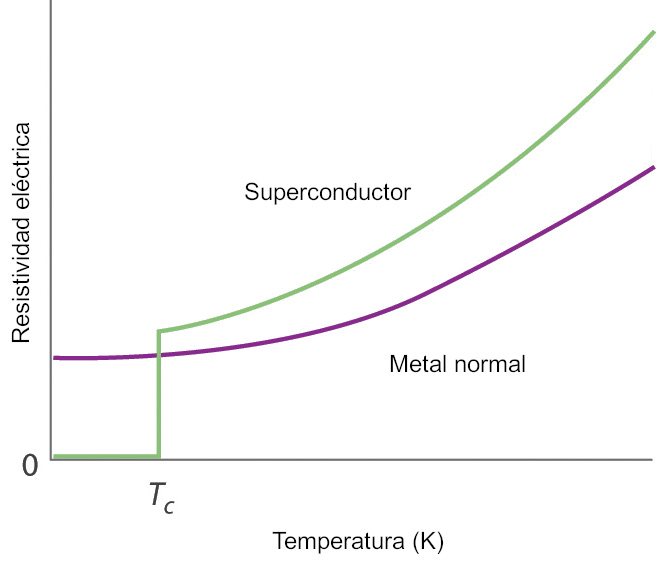
\includegraphics[scale=1.5]{Imagenes/Superconductividad_01.jpg}
\end{figure}
\end{frame}

\subsection{Aplicaciones}

\begin{frame}
\frametitle{Aplicación del superconductor}
La superconductividad tiene numerosas aplicaciones tecnológicas:
\pause
\setbeamercolor{item projected}{bg=cadet,fg=black}
\setbeamertemplate{enumerate items}{%
\usebeamercolor[bg]{item projected}%
\raisebox{1.5pt}{\colorbox{bg}{\color{fg}\footnotesize\insertenumlabel}}%
}
\begin{enumerate}[<+->]
\item Creación de imanes superconductores para la resonancia magnética nuclear (RMN) y la resonancia magnética (RM) en medicina.
\seti
\end{enumerate}
\end{frame}
\begin{frame}
\frametitle{Aplicación del superconductor}
La superconductividad tiene numerosas aplicaciones tecnológicas:
\pause
\setbeamercolor{item projected}{bg=cadet,fg=black}
\setbeamertemplate{enumerate items}{%
\usebeamercolor[bg]{item projected}%
\raisebox{1.5pt}{\colorbox{bg}{\color{fg}\footnotesize\insertenumlabel}}%
}
\begin{enumerate}[<+->]
\conti
\item Transmisión de energía eléctrica sin pérdidas.
\item Aceleradores de partículas.
\item Fabricación de dispositivos electrónicos de alta sensibilidad, como detectores de radiación.
\end{enumerate}
\end{frame}

\end{document}